%调整图片与上方文字之间的间距
%\vspace{-0.1cm}
\begin{figure}[h]
	\vspace{6pt} % 图:段前距 6 磅
	\centering
	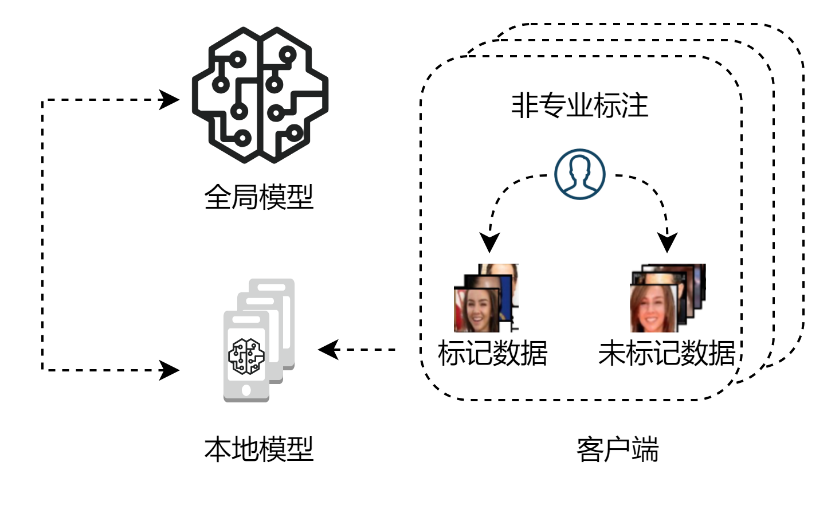
\includegraphics[width=10cm]{chapters/imgs/LabelAtClient}
	
	% 使用bicaption设置双语图题,调整行距为20磅
	\begingroup
	\setlength{\baselineskip}{20pt} % 设置行距为20磅
	
	% 中文图题:宋体,五号,段前距6磅,段后距0磅
	\vspace{6pt}
	\bicaption[\xiaosi 标记数据在客户端的情况]
	{\songti\wuhao 标记数据在客户端的情况} % 中文图题:宋体,五号
	{\rmfamily\wuhao Labeled data on the client side} % 英文图题:Times New Roman,五号
	
	% 英文图题:段后距12磅
	\vspace{0pt}
	\endgroup
	
	\label{LabelAtClient}
\end{figure}
%调整图片与下方文字之间的间距
\vspace{-0.35cm}



%调整图片与上方文字之间的间距
%\vspace{-0.1cm}
\begin{figure}[h]
	\vspace{6pt} % 图:段前距 6 磅
	\centering
	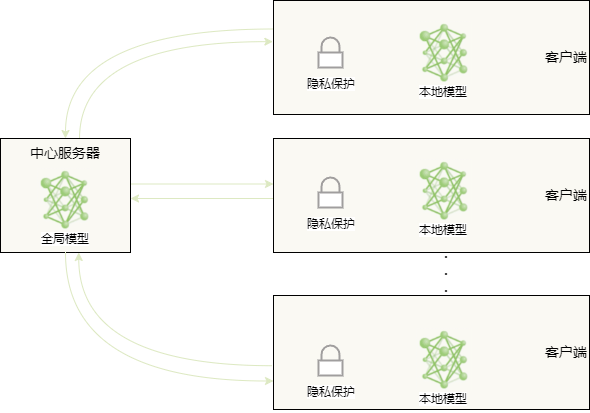
\includegraphics[width=10cm]{chapters/imgs/FedArch3} % 插入图像,设置图像的宽度为10cm
	
	% 使用bicaption设置双语图题,调整行距为20磅
	\begingroup
	\setlength{\baselineskip}{20pt} % 设置行距为20磅
	
	% 中文图题:宋体,五号,段前距6磅,段后距0磅
	\vspace{6pt}
	\bicaption[\xiaosi 联邦学习系统架构] % 设置双语标题,括号中的部分是用于生成目录中的标题,设置为“小四号字体”,标题内容是“不同缩放系数v的缩放效果”
	{\wuhao 联邦学习系统架构} % 中文标题,设置字体为“无号”并且标题内容为“标记数据在客户端的情况”
	{\wuhao Federated learning system architecture} % 英文标题,设置字体为“无号”并且标题内容为“Labeled the data on the client side”
	
	% 英文图题:段后距12磅
	\vspace{0pt}
	\endgroup
	
	\label{FedArch} % 给图形一个标签,便于在文档中引用,标签为 "fig:3.1"
\end{figure}
%调整图片与下方文字之间的间距
\vspace{-0.35cm}




\begin{table}[h]
	
	\centering  % 表格居中
	% 双语标题,其中中文部分用了 \songti 与 \wuhao
	\bicaption[\xiaosi \songti 联邦半监督学习方法总]
	{\songti \wuhao 联邦半监督学习方法总结}
	{\songti \wuhao Summary of federated semi-supervised learning methods}
	\label{SummaryOfFedSemi}
	
	% 使用 \resizebox 命令缩放表格到页面宽度
	\resizebox{\textwidth}{!}{
		% 整体使用 {\songti \wuhao ...} 包裹表格内容
		{\songti \wuhao
			\begin{tabular}{cccccc}
				\toprule[1.5pt]
				类别 & 方法 & 半监督学习算法 & 隐私保护方案 & 数据异质问题 & 性能 \\
				\midrule[0.75pt]
				\multirow{6}{*}{标签在客户端} 
				& RSCFed     & 教师学生模型 & 无     & 加权距离聚合   & 无                \\
				& FedSSL     & 伪标记       & 差分隐私 & 全局生成模型     & 无               \\
				& FedMatch   & 伪标记       & 无     & 客户端间一致性  & 分散学习和稀疏学习 \\
				& FedPU      & PU Learning  & 无     & 客户端间一致性  & 无                \\
				& AdaFedSemi & 伪标记       & 无     & 无             & 调整置信度阈值和参与率 \\
				& DS-FL      & 集成未标记   & 无     & 无             & 传输日志、无参数     \\
				\midrule
				\multirow{2}{*}{标签在服务器端} 
				& SemiFL     & 伪标记       & 无     & 减少熵的平均值   &                   \\
				& FedMatch   & 伪标记       & 无     & 客户端间一致性   & 分散学习和稀疏学习   \\
				\bottomrule[0.75pt]
			\end{tabular}
		}
	}
\end{table}